\documentclass[assignment06_Solutions]{subfiles}

\IfSubStr{\jobname}{\detokenize{Solutions}}{\toggletrue{solutions}}{\togglefalse{solutions}}

\fancypagestyle{firstpage}

{\rhead{Assignment 6 \linebreak \textit{Version: \today}}}

\title{Assignment 6: Introduction to Neural Networks and Backpropagation}
\author{Machine Learning}
\date{Fall 2019}

\begin{document}

\maketitle
\thispagestyle{firstpage}


\begin{learningobjectives}
\bi
\item Gain some familiarity with some of the key ideas in machine learning.
\item Review of mathematical concepts we will be using in the beginning part of this course.
\item Familiarize yourself with computational tools for machine learning.
\item Learn linear regression using a ``top-down'' approach.
\ei
\end{learningobjectives}


\href{https://www.math.hmc.edu/calculus/tutorials/multichainrule/}{HMC Multivariable Chain Rule Page}
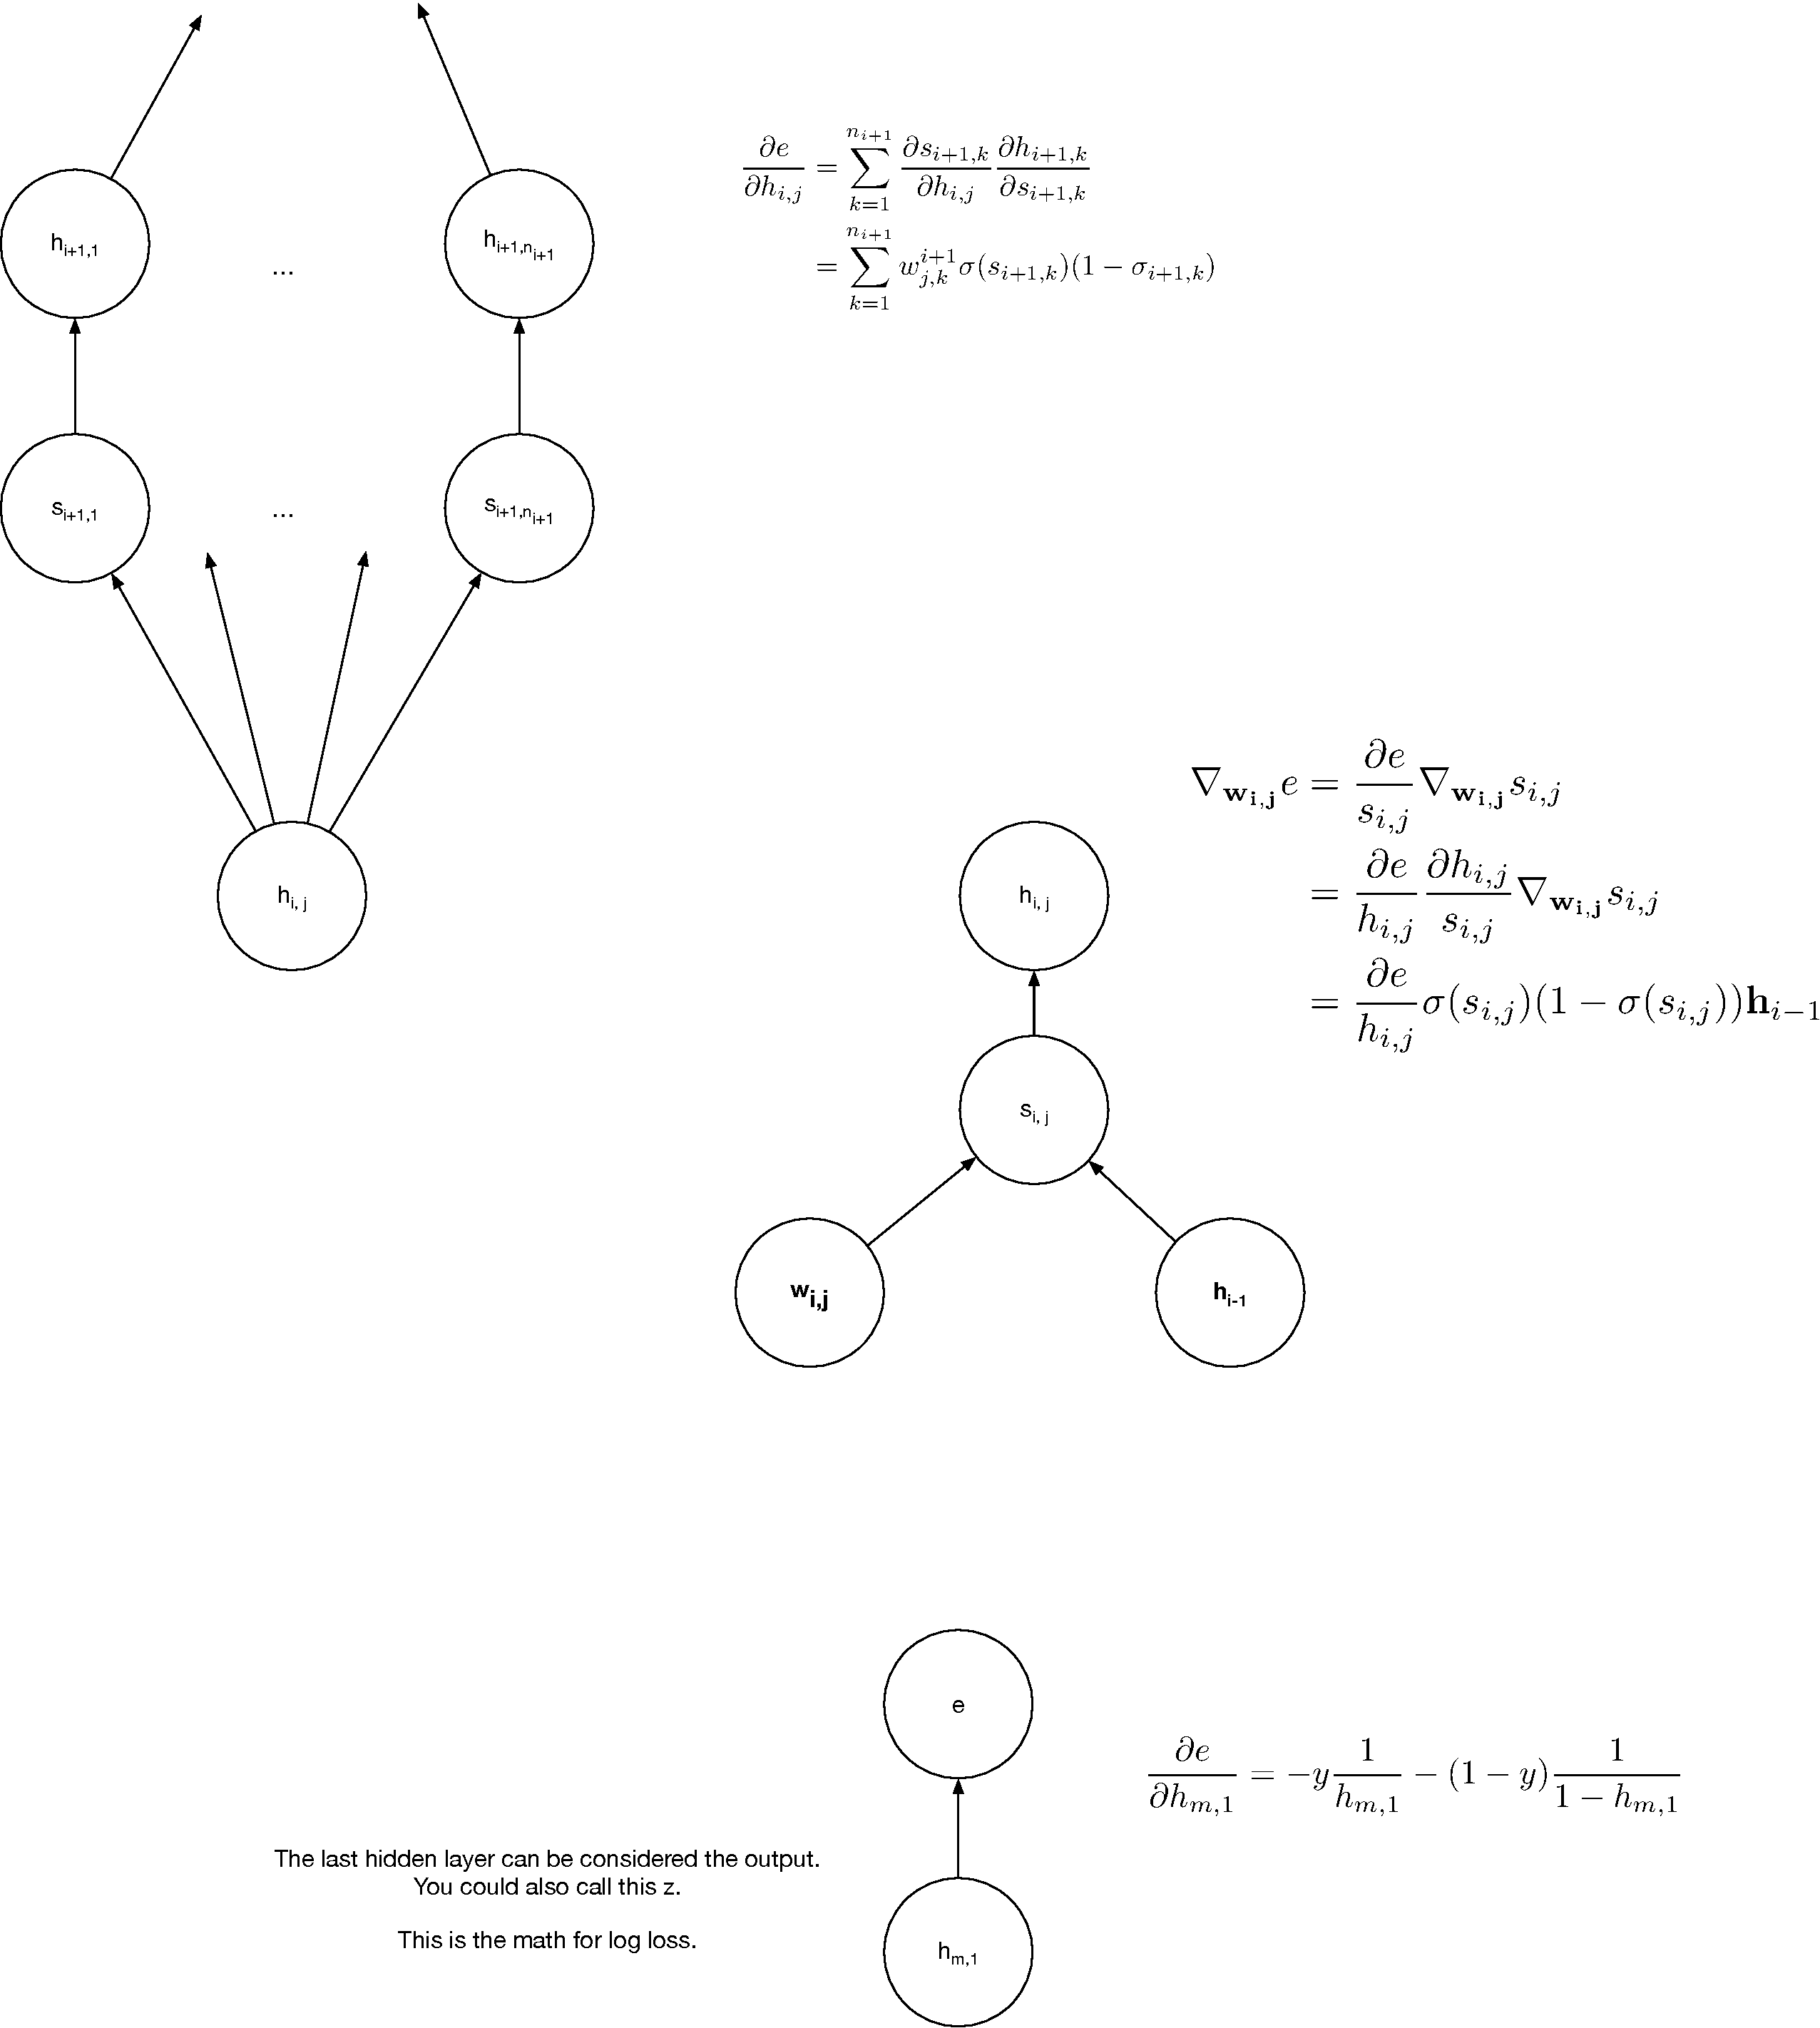
\includegraphics[width=\linewidth]{figures/singleneuroncloseup}
Todo: use a variable for layer instead of just hidden (this would simplify things).

Hidden unit to error:
\begin{align}
\frac{\partial{e}}{\partial{h_{i,j}}} &= \sum_{k=1}^{n_{i+1}} \frac{\partial s_{i+1, k}}{\partial h_{i,j}} \frac{\partial h_{i+1, k}}{\partial s_{i+1, k}} \frac{\partial e}{\partial h_{i+1, k}} \\
&= \sum_{k=1}^{n_{i+1}} w^{i+1}_{j,k} \sigma(s_{i+1,k})(1 - \sigma_{i+1,k})\frac{\partial e}{\partial h_{i+1, k}}
\end{align}

Weights to error:
\begin{align}
\nabla_{\mathbf{w_{i,j}}} e &= \frac{\partial e} {s_{i,j}} \nabla_{\mathbf{w_{i,j}}} s_{i,j} \\
&= \frac{\partial e}{h_{i,j}}  \frac{\partial h_{i,j}}{s_{i,j}} \nabla_{\mathbf{w_{i,j}}} s_{i,j} \\
&= \frac{\partial e}{h_{i,j}}  \sigma(s_{i,j})(1-\sigma (s_{i,j})) \mathbf{h}_{i-1} 
\end{align}

Output to error (serves as a base case.  For simplicity we use $h_{m,1}$ to refer to the single node in the $m$th layer (which is the output layer).
\begin{align}
\frac{\partial{e}}{\partial h_{m,1}} = - y \frac{1}{h_{m,1}} - (1-y) \frac{1}{1-h_{m,1}}
\end{align}

\end{document}
